
\begin{frame}[t,allowframebreaks]{Introduction to regularisation -}

The `no free lunch' theorem of \gls{ml} implies that we
need to design our algorithms 
to perform well on \underline{specific tasks}.

\vspace{0.2cm}

We do this, for example, by:
\begin{itemize}
    \item adjusting the algorithm's 
    \index{representational capacity}\gls{representational capacity}, or by    
    \item giving an algorithm a 
    {\bf preference for some type of solution}.
\end{itemize}

\vspace{0.1cm}

\begin{blockexample}{}
\begin{itemize}
    \small
    \item 
    Non-preferred solutions are penalised but remain eligible.
    \item 
    A non-preferred solution can still be chosen if it fits the training 
    data significantly better than the preferred one.
\end{itemize}
\end{blockexample}

\vspace{0.3cm}

There exist several {\bf strategies to reduce the test/generalisation error},
possibly at the price of increasing the training error.\\
\vspace{0.2cm}

These strategies are {\bf referred to collectively as
\index{regularisation}\gls{regularisation}}.


\framebreak

%
%

A simple form of \index{regularisation}\gls{regularisation} is 
\index{weight decay}\gls{weight decay}.\\
\vspace{0.2cm}

We can modify the loss function, $L(\vect{w})$, 
to include a \index{regulariser}\gls{regulariser} $\Omega(\vect{w})$:
\begin{equation}
    L(\vect{w}) \rightarrow L(\vect{w}) + \Omega(\vect{w})
    %\label{eq:}
\end{equation}\\

The \gls{regulariser} has the form:
\begin{equation}
    \Omega(\vect{w}) = \lambda \vect{w}^T \vect{w} 
    %\label{eq:}
\end{equation}\\

and expresses a {\bf preference for the weights to have a smaller $L^2$ norm}.\\
\vspace{0.1cm}
The factor $\lambda$ is fixed prior to training and controls the
strength of our preference for smaller weights.
\vspace{0.2cm}

Minimising $L(\vect{w})$ results in a tradeoff, 
in the choice of $\vect{w}$, between:
\begin{itemize}
\item fitting the training data, and
\item being small.
\end{itemize}

\framebreak

%
%

The \index{regulariser}\gls{regulariser}
$\Omega(\vect{w})$ controls 
a model's tendency to overfit or underfit.\\
\vspace{0.2cm}
Increasing $\lambda$, forces the model to {\bf put weight
on fewer features}.\\
\vspace{0.2cm}
A preference for smaller weights, {\bf decreases the model variance}.
\begin{itemize}
    \small
    \item
    Similar solutions will be preferred for 
    different training sets from the same data-generating distribution.
\end{itemize}

\begin{columns}
    \begin{column}{0.72\textwidth}
        \begin{center}
            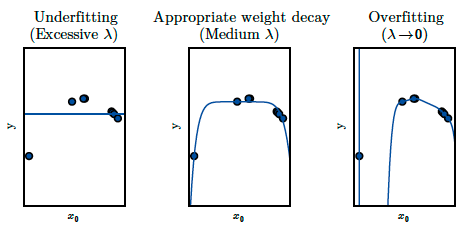
\includegraphics[width=0.99\textwidth]
                {./images/training_issues/goodfellow17_regularisation_weigh_decay_example_1.png}\\
            \vspace{0.0cm}
            {\tiny 
                Using weight decay to control a model's tendency to overfit or underfit.\\
                \color{col:attribution} 
                Schematic reproduced from p. 116 of \cite{Goodfellow:2017MITDL}.\\
            }
        \end{center}        
    \end{column}
    \begin{column}{0.28\textwidth}
        {\scriptsize
        The example on the left, 
        shows the impact of different values of $\lambda$ 
        on the result of training a high-degree (degree 9) 
        polynomial regression model
        to examples from a quadratic data-generating distribution.\\
        }
    \end{column}
\end{columns}

\framebreak

%
%

Several \index{regularisation}\gls{regularisation} 
techniques are known to \gls{ml} practitioners.\\
\vspace{0.3cm}

Broadly speaking, we can distinguish between techniques that:\\
\vspace{0.1cm}
\begin{itemize}
    \item 
    {\bf modify the \index{loss function}\gls{loss function}}
    \begin{itemize}
        \item e.g. L1 and L1 \gls{regularisation} (Lasso and Ridge), entropy
    \end{itemize}
    \vspace{0.1cm}
    \item
    {\bf modify the data sampling method}
    \begin{itemize}
        \item e.g. data augmentation, k-fold cross-validation
    \end{itemize}
    \vspace{0.1cm}
    \item
    {\bf modify the training method}
    \begin{itemize}
        \item e.g. noise injection, dropout
    \end{itemize}
\end{itemize}

\vspace{0.3cm}

We will have a closer look at \gls{regularisation} 
techniques later in Part {\thispart}.\\

\end{frame}